\chapter[Vertical Drift Chambers]{Vertical Drift Chambers
\footnote{
  $CVS~revision~ $Id: vdc.tex,v 1.5 2003/12/05 07:12:10 gen Exp $ $
}
\footnote{Authors: J.Segal \url{mailto:segal@jlab.org}}
}
% This section written by K.G. Fissum in January 1997.
% V2.0 - OSP for ArC2H6 VDC use
% Direct all comments/questions to:
% fissum@cebaf.gov
% TJNAF Room 16-125
% (757) 269 7325

% modified as per Bogdan's request 3/24 for new
% ops manual - changed responsible personel

% modified after catching some errors 
% updated some figures 990825
% KF kevin.fissum@nuclear.lu.se

% minor modifications  031113
% changed responsible personnel
% Bertan supplies are modified for remote reset
% fans are now mounted in VDC faraday cage cover
% HAWGS is now incorporated in HAGS
% gas system status is now logged automatically in EPICS
% JS segal@jlab.org

\section{Overview}

The High Resolution Spectrometer Vertical Drift Chambers provide a
precise ($\pm 125~\mu$m) measurement of the position and angle of
incidence of both recoil electrons (in the HRSe) and knockout protons
(in the HRSh) at the respective spectrometer focal planes.  This
information may be combined with the knowledge of the spectrometer
optics to determine the position and angle of the particles in the
target.

Each Hall A spectrometer boasts its own VDC detector package.  These
packages are located on permanent rails mounted on the spectrometer
decks in the shielding huts above the outrun windows but beneath the
space frames.  The packages consist of two VDCs, and are identical
in all aspects.  The VDCs have been constructed without guard wires.
Each VDC is composed of two wire planes in a standard UV
configuration - the wires of each plane are oriented at 90$^\circ$
to one another, and each plane is oriented at 45$^\circ$ with respect
to the nominal particle trajectories (see Figures
\ref{fig:trajectory1},\ref{fig:trajectory2}).

\begin{figure}
\begin{center}
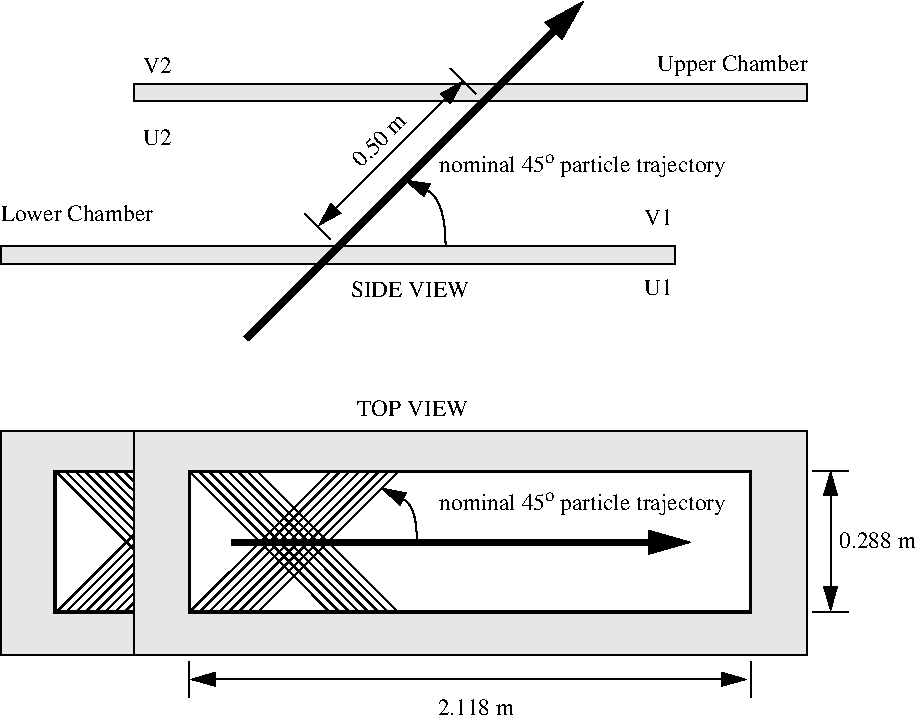
\includegraphics[angle=0,width=0.7\textwidth,clip]{vdc_geom_1}
\caption[Detectors: VDC Geometry]{Relative VDC geometry}
\label{fig:trajectory1}
\end{center}
\end{figure}

\begin{figure}
\begin{center}
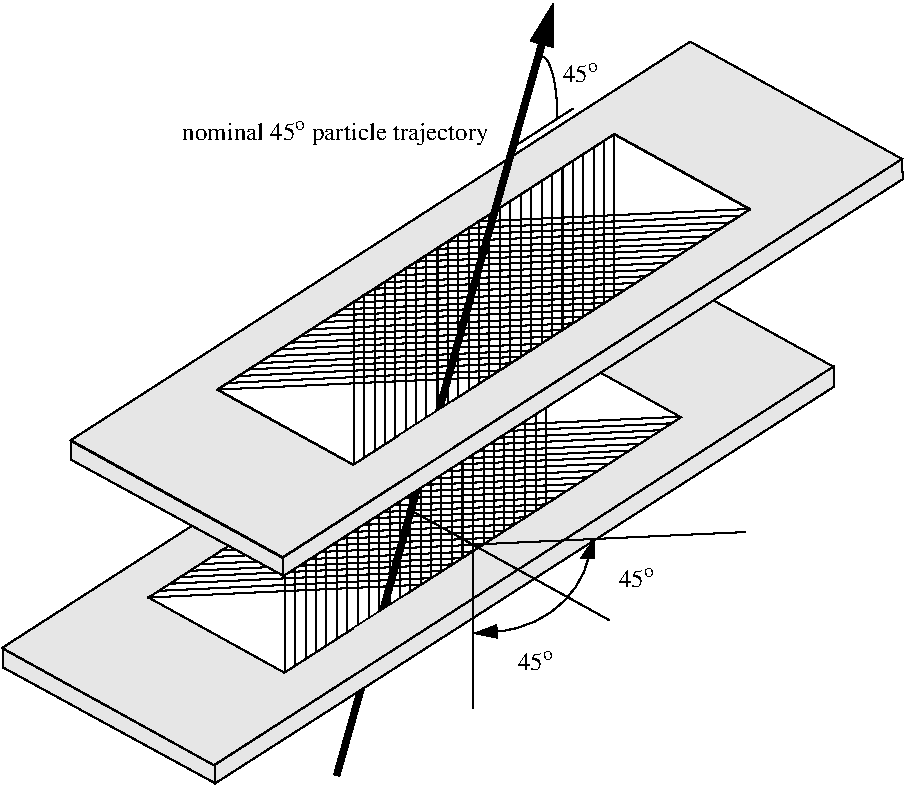
\includegraphics[angle=0,width=0.7\textwidth,clip]{vdc_geom_2}
\caption[Detectors: VDC Geometry]{Relative VDC geometry}
\label{fig:trajectory2}
\end{center}
\end{figure}

Operation of the VDCs requires the application of both High Voltage
(HV) across the chambers themselves and Low Voltage (LV) across the
preamp/disc cards, which are mounted on the sides of 
the VDCs, within the confines of the protective aluminum Faraday cage.
The chamber gas is a combination of argon (Ar) and flammable ethane
(C$_2$H$_6$) which is bubbled through alcohol.  Gas is routed from
bottles located in the Hall A gas supply shed to gas supply control
panels located on the main level of the space frames in the detector
huts.

\infolevthree{
As charged particles pass through the chamber gas in the VDCs, they
produce ionization.  This ionization drifts along the electric field
lines defined by the high voltage planes and the signal wires.  
Ionization is collected in the form of analog pulses on the signal
wires.  The pulses are then amplified, discriminated and used to
start multihit TDCs, which are subsequently stopped by the overall
event trigger.  The TDCs are read out by the CODA\cite{CODAwww} acquisition
software.  The data are histogrammed online by the \mycomp{dhist} 
(see Sec.~\ref{sec:onl-dhist}) software.  In-depth data analysis  
requires the offline software (see Sec.~\ref{sec:onl-ofl-analysis}).
} %infolev
\infolevtwo{
\section{Operating Procedure}
\paragraph {Gas Flow Operating Procedures}

Chamber gas is delivered to a given VDC detector package via HAGS,
the Hall A Gas System.  Complete details of this system
are presented elsewhere in this manual.

Each VDC detector package consists of two VDCs connected in parallel
(see Figure \ref{fig:gasflow}).  All gas connections are made using
Polyflo$\rm ^{TM}$ tubing and Jefferson Lab specified connectors.  Gas 
enters the chamber assembly after bypassing an overpressure bubbler 
containing 15 mm of (edible) mineral oil.  Gas is exhausted from the 
VDC package through a second bubbler containing 5 mm of mineral oil.
Each chamber has a volume of approximately 30 $\ell$ and is operated
slightly above atmospheric pressure.  Standard flow rate set points
are clearly labeled next to the control panel flow meters.  The gas
flow through the chambers may be independently varied and is typically
set to 7 $\ell$/hr.  A typical chamber leakage rate measured against 
the 5-mm mineral oil load is $\le$ 3 $\ell$/hr.  The flow rate of
7 $\ell$/hr when combined with the leak rate of $\le$ 3 $\ell$/hr
ensures a complete exchange of gas in the chambers roughly every
8 hours. When a
bottle is nearly empty (say 90\%), it should be changed since the
quality of the gas at the bottom tends to be low.  Gas bottles may
only be changed by authorized personnel.


\begin{figure}
\begin{center}
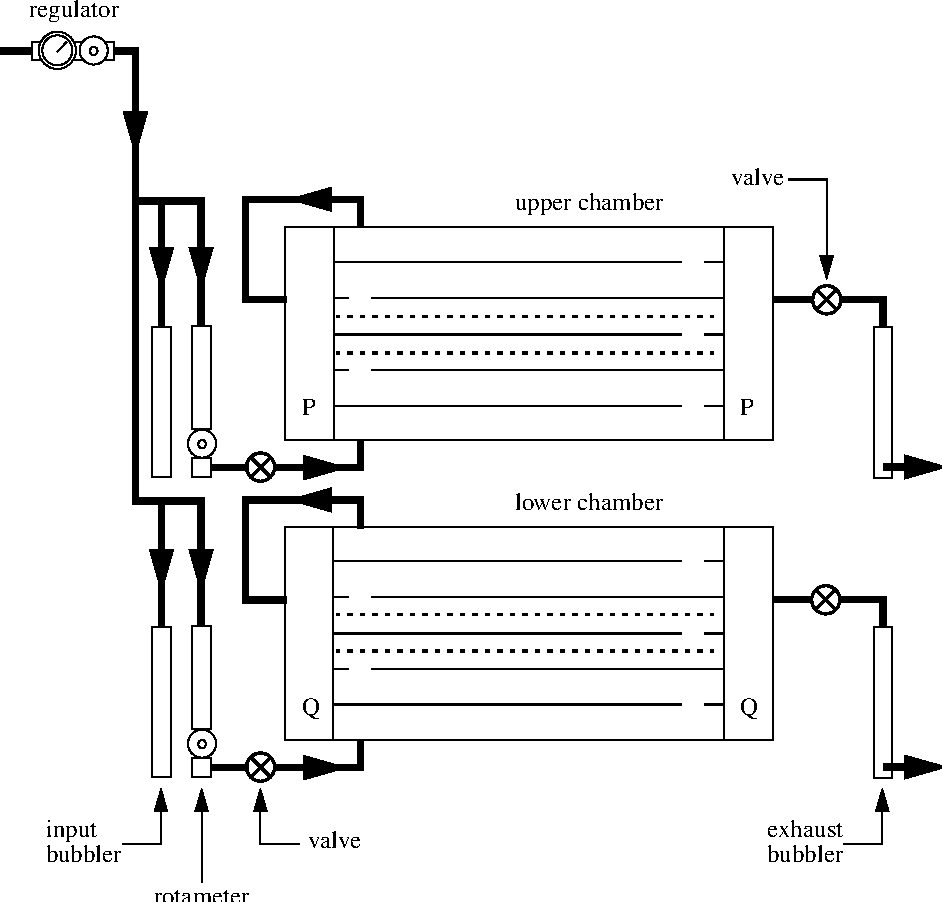
\includegraphics[angle=0,width=0.7\textwidth,clip]{vdc_gasflow}
{\linespread{1.}
\caption[Detectors: Gas Flow Schematic]{Gas flow schematic}
\label{fig:gasflow}}
\end{center}
\end{figure}

The status of the gas handling system should be monitored carefully
every shift.  Manual logging is not required as the system status is
constantly logged via EPICS~\cite{EPICSwww}.  Any substantial deviation from the
median parameters can result in a change in the operational parameters
of the VDCs and should be immediately investigated.  If at all
possible, gas flow should be continuously maintained, even in
no-beam time periods.   This avoids time loss to reconditioning and
maintains the desirable steady-state operating condition.  Further,
it is critical that gas flow has been maintained for 24 hours prior
to any power up.

\paragraph{Power Supplies and Electronics Procedures}
\label{lv}

The power supplies and readout electronics associated with the HRS
VDCs are all commercially designed.  The reader is directed towards
the manuals made available by the manufacturer for the detailed
information not provided here.


\begin{figure}
\begin{center}
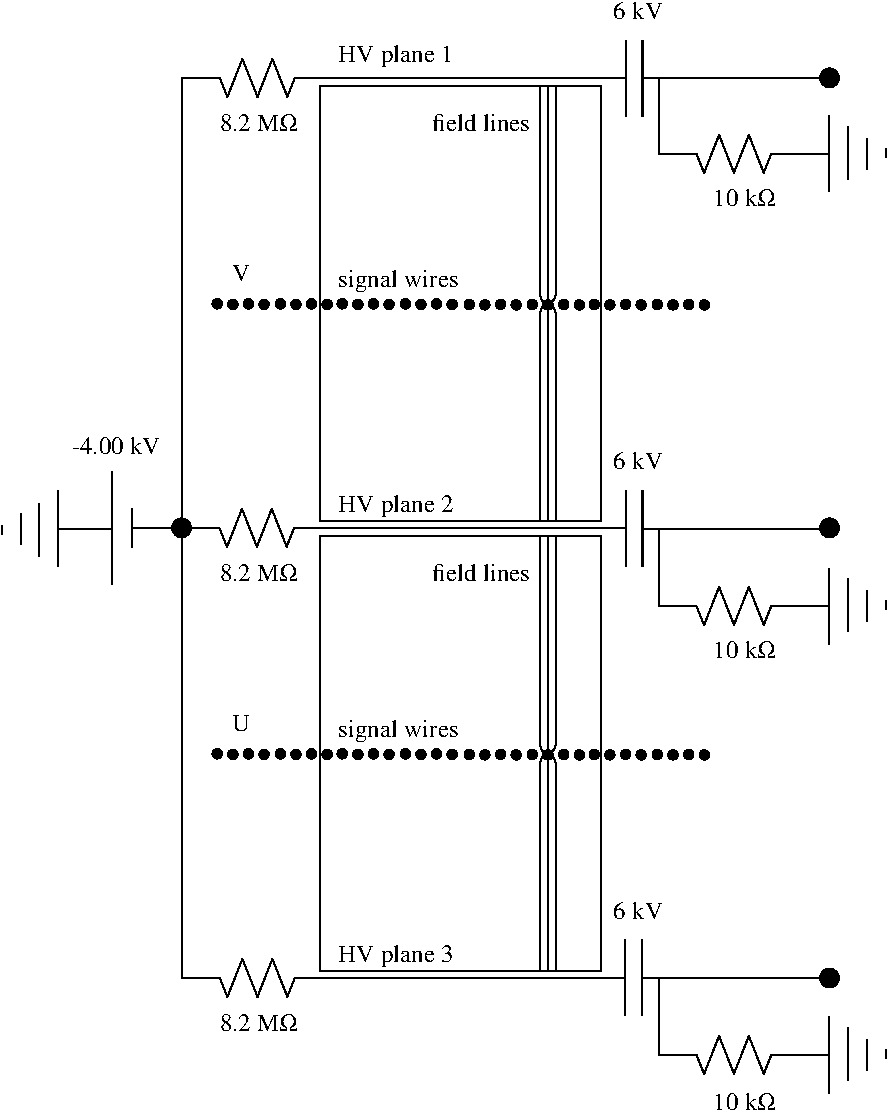
\includegraphics[angle=0,width=0.6\textwidth,clip]{vdc_scheme}
\caption[Detectors: VDC Overview]{VDC overview.}
\label{fig:vdcscheme}
\end{center}
\end{figure}

A Bertan 377N HV power supply, modified to allow a remote reset,
provides -4.00 kV nominal to
each of three HV planes in a given VDC detector package via a
10 M$\Omega$ Hammond splitter box (see Figure \ref{fig:vdcscheme}).
The power supply is located in
the detector hut in a NIM bin on the upper level of the space frame.
This unit may be controlled either manually or remotely via the
EPICS control software, and also provides a monitor of the
current drawn (nominally 70 nA) by the VDCs to which it is attached.
Connections from the power supply to the Hammond splitter box, as
well as from the Hammond splitter box to the VDCs are made using
standard SHV connectors on red RG-59/U cable good to 5 kV.

A Kepco ATE 15-3m discriminator power supply provides +3.0 V (92 cards
draw $\leq$ 2 A) and the Kepco ATE 6-100m pre-amp power supply provides 
$\pm$5 V nominal to the LeCroy 2735DC pre-amp/discriminator cards used 
to instrument the chambers via a heavy-duty fuse panel.  The precise 
voltages provided are +5.0 V (92 cards draw 22 A) and -5.2 V (92 cards 
draw 58 A).  These LV supplies are located in the detector hut on the 
main level of the space frame for the HRS$_{\rm e}$ and on the upper 
level of the space frame for the HRS$_{\rm h}$.
Complete connection schematics and instructions
for making or breaking the connections are located on the aluminum
Faraday cage protective plates covering the respective interface
nodes between the power supplies and the VDCs.

Each VDC wire plane consists of 400 20 $\mu$m $\phi$, Au-plated
tungsten wires.  The first 16 wires on each end of the wire plane
are connected to ground for field-shaping purposes.  There are
368 wires per wire plane which act as signal wires.  Thus, each
spectrometer is instrumented with 1472 channels of LeCroy 1877
multihit Fastbus TDCs.  These TDCs are located in a Kinetic Systems
F050 Fastbus crate with a BiRa FB8189-4 power supply located on the 
main level of the spectrometer space frame in
the detector hut.  The connections between the pre-amp/discriminator
cards mounted on the VDCs and the TDCs are made with 34-conductor
twisted-pair cables.  Clip-on ferrites are used to filter noise.
A connection schematic is posted on the side of the rack holding
the Fastbus crate on the space frame in the detector hut.

\begin{center}
{\bf Power-up Procedure}
\end{center}

\begin{enumerate}
\item {ensure gas flow has been established in the chambers as
previously outlined.  If it has not, {\it STOP RIGHT
HERE!}  Gas flow must be well-established and steady-state
{\it BEFORE} the HV may be enabled.}
\item {Ensure that all power supplies as well as the Fastbus crate
are off and then connect the LV, HV, and TDC cables.}
\item {enable the LV.  Set points are clearly labeled on the face of
the power supplies.  Note that they have overcurrent setpoints, and
some fine adjustments over the first 30 minutes after a cold start
power-up may be required.  Appropriate LEDs should all be active on
both the power supplies and the pre-amp/discriminator cards.}
\item {slowly (steps of no more than -300 V) ramp the HV to its
nominal set point of -4.00 kV using either the manual or the remote
controls.  While the trip current is set to 10 $\mu$A, do not allow
the chambers to draw more than 1 $\mu$A during the ramping procedure
or serious damage may result.  If the power supply trips during the
ramping procedure, you are moving too fast.  Rezero things and begin
the procedure again.  {\it NEVER USE THE AUTO-RESET FUNCTION.}}  If
the power supply trips again, {\it STOP IMMEDIATELY AND INVESTIGATE.}
\item {enable the Fastbus crate.  Appropriate LEDs should all be
active.}
\item {check for poor signal connections evidenced by hot wires (wires
counting extremely fast) or dead wires (wires with no counts) using
the histograming software and cosmic rays.  Remake any connections as
necessary by first powering down the Fastbus crate.}
\end{enumerate}

If at all possible, the HV and LV power supplies should be left
on continuously if and only if gas is available to the chamber.  This
avoids time loss to reconditioning and maintains the desirable
steady-state operating condition.

\section{Handling Considerations}

The VDCs are very delicate devices which are absolutely essential to
the instrumentation of the Hall A spectrometers.  Thus, extreme care
must be exercised whenever they are moved or used.

\begin{itemize}
\item{Before moving a VDC detector package, ensure that the protective
plates are in position.  Plates include tapped aluminum sheets to
be bolted over the entrance and exit aperatures, as well as aluminum
sheets which slide in between the two chambers.}
\item{Disconnect and reconnect all TDC cables with extreme care.  The
conductor pins are relatively fragile, and should one be broken off,
repair will be {\it extremely} difficult.}
\item{When initiating gas flow, pay strict attention to the feedback
parameters.  Overpressure may damage the chambers.}
\item{Never attempt to apply HV to the chambers until gas flow
conditions have reached steady-state.}
\item{As the amount of heat generated by the pre-amp/discriminator
cards it substantial, always make sure adequate cooling is provided
before attempting to run.  This cooling takes the form of
four 12VDC fans mounted in the aluminum Faraday cage.}
\item{When ramping the HV, never allow the chambers to draw more than
1 $\mu$A instantaneously.  If they do, something is wrong!}
\end{itemize}

\section{Other Documentation}
See the URL%
\htmladdnormallinkfoot{}{\url{
http://www.jlab.org/~fissum/vdcs.html
}}.
} %infolev

\begin{safetyen}{5}{5}
\section{Safety Assessment}
The following potential hazards have been clearly identified.
\end{safetyen}
\begin{description}
\item {\bf The High Voltage System}
The Bertan 377N HV low current power supply provides a nominal
-4.00 kV.  Red HV RG-59/U cable good to 5 kV with standard SHV
connectors is used to connect the power supply to a Hammond splitter
box, and then to connect the splitter box to each of the three high
voltage planes in a given VDC.  A given chamber draws a current
from  50-100 nA.
\item {\bf The Low Voltage System}
Kepco LV power supplies are used for the the LeCroy 2735DC
pre-amp/discriminator cards.  Each card (23 per chamber) requires
+5.0 V (92 cards draw 22 A), -5.2 V (92 cards draw 58 A) and +3.0 V
(92 cards draw $\leq$ 2 A).
\item{\bf Explosive Gas} The Ar~C$_2$H$_6$ chamber gas is explosive
and must be handled accordingly.  Further, gas flow should be maintained
for at least 24 hours prior to the enabling of HV.
\item{\bf High Pressure Gas Bottles} The gas used in the chambers
is supplied in high pressure ($\ge$ 2000 psi) gas bottles. This
confined high pressure gas represents a tremendous (potentially lethal)
amount of stored energy.
\end{description}

\section{Responsible Personnel} 
\label{people}
The following individuals are responsible for chamber problems. 
\begin{itemize} 
\item[~]Segal, Jack - x7242, pager 584-7242 
\item[~]Wojtsekhowski, Bogdan - x7191, pager 584-7191 
\end{itemize} 

% ===========  CVS info
% $Header: /group/halla/analysis/cvs/tex/osp/src/hrs_det/vdc.tex,v 1.5 2003/12/05 07:12:10 gen Exp $
% $Id: vdc.tex,v 1.5 2003/12/05 07:12:10 gen Exp $
% $Author: gen $
% $Date: 2003/12/05 07:12:10 $
% $Name:  $
% $Locker:  $
% $Log: vdc.tex,v $
% Revision 1.5  2003/12/05 07:12:10  gen
% shower.tex modified. infolevel added. Polishing
%
% Revision 1.4  2003/11/13 21:35:26  gen
% Correction from Jack
%
% Revision 1.3  2003/06/06 17:00:27  gen
% Revision printout changed
%
% Revision 1.2  2003/06/05 23:30:01  gen
% Revision ID is printed in TeX
%
% Revision 1.1.1.1  2003/06/05 17:28:30  gen
% Imported from /home/gen/tex/OSP
%
%  Revision parameters to appear on the output
